%parent: main.tex
\section{Testing and Evaluation}
\label{eval}
We have considered multiple approaches for the Testing and Evaluation phase. A detailed discussion is presented in the following section. 
%\newline
\subsection{Training on full svcomp14 and testing on full svcomp15}
 Svcomp15 had changes in its method of score assignment and evaluation strategies in comparison to svcomp14. Moreover, there were a bunch of new tools, $T_{new}$, that participated in svcomp15 , not present in svcomp14, while there are also a set of tools, $T_{old}$, that participated in 2014 but are absent in 2015. Since we have learnt based on the data of 2014, we only have learned predictors for the set of 2014. Hence, from the 2015 data-set we have curtailed out the new tools, while the old tools that did not participate at all are treated as non-participating, that is, their scoring is set to a low value beyond the minimum normalized score as discussed earlier. This leads to the fact that predictions using the 2014 based learned predictors will not match the svcomp reported results of 2015 over various categories. However, we feel there are two valuable aspects that we can focus on while comparing our predicted results with that of svcomp15. Firstly, how well the $T_{old}$ would have performed if they had participated, and secondly, for tools that participated in both , has there been an improvement in the tool's performance from the previous year? \newline
 For the first question, we get interesting results. 
As shown in the Figure \ref{fig:test_nonlin_15}, LLBMC did participate in svcomp14, but not in svcomp15. That acquired the third rank in svcomp14, and it is expected that it could be ranked as second winner if it had participated. Also, CPAChecker is our predicted winner, that matches with the published results on svcomp15. The tool CBMC came third in svcomp15, whereas our prediction shows it in the forth position closely competing by ESBMC. This slight deviation is expected since we do not consider the runtime of the tools unlike the actual competition. The graphs in the svcomp15 website shows those two tools to be closely competing as well.

 For the latter case as well, we see interesting deviations. In svcomp15 UltimateAutomizer came to be in the second position, however our prediction shows it to be one of the least preferred tools. This is because in svcomp14 it performed poorly compared to other tools, and hence according to our learned predictor, it ranks below most of the tools. That suggests this tool possibly has been improved.
 
\begin{figure}
	\label{fig:test_nonlin_15}
	\centering
	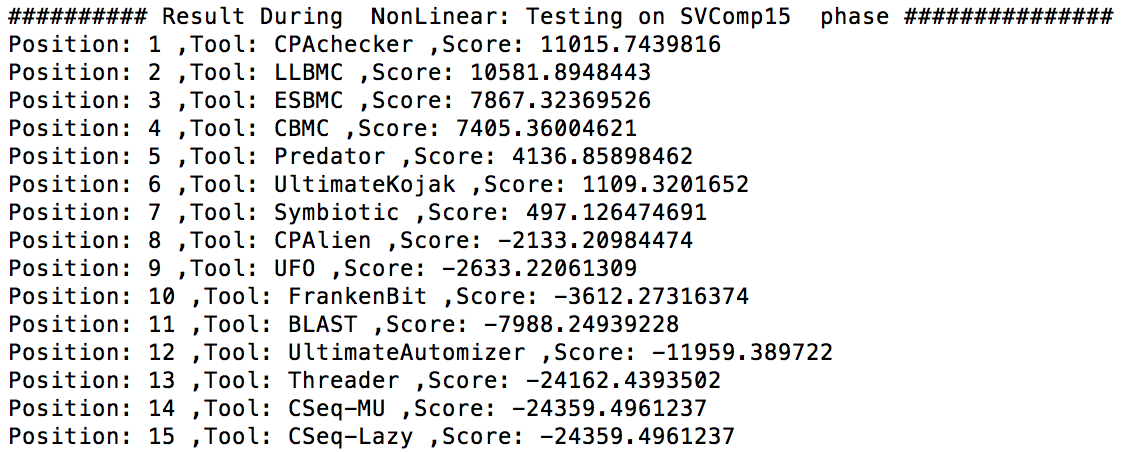
\includegraphics[width = 4.5in]{figures/test15.PNG}
	\caption{Testing on SVComp15 data using learned prediction on SVComp14}
\end{figure} 
 
 %\textbf {NonLinear Regression: With regulariser}
 \subsection{Partitioning SVComp14 as training and test data}
 This is in accordance to the method followed in [1]. Since there is a mismatch in scoring mechanisms between svcomp14 and svcomp15, and also the possible improvements that has been implemented in the participating tools over the year. Hence, in this method we choose svcomp14 as the complete data for both training and testing. To make sure that test data is never seen during the training phase, we perform a randomized split of the data in a $60:40$ ratio(following[1]) such that a random $60\%$ becomes the $train_{14}$ data and the remaining $40\%$ becomes the $test_{14}$ data. Since the partitioning is randomized, we repeat this mechanism 5 times and report the arithmetic mean of the training and test accuracies. In this case as well, we perform cross validation over the regularizer component ($\lambda$) and choose the best one for each tool that determines the final hypothesis for that tool. Since, this is a regression problem, unlike the classification problem of dividing into half-spaces, we have chosen relative error as the measure of accuracy. The relative error is the relative deviations of the predictions from the true score in the test set. The tolerance is chosen to be in $\pm 5\%$ for the reported data. We did try out tighter bounds on accuracy of within $\pm 1\%$, but that gives extremely low accuracy, indicating the fit of the predictor to be within the $5\%$ band of the true score. Our analysis suggest that a looser band is expected since the test label being compared with had an initial approximation of getting the score of its corresponding category and not the exact score it would have had on running over the tools. This we assumed to be a reasonable approximation since benchmarks within a category are expected to resemble closely related feature values and hence should expect similar score. Figure \ref{fig:test_14} shows the accuracy of every tool based on this approach using both basic linear regression and using non-linear transformation with regularization.
 
 \begin{figure}
\centering
\begin{tabular}{c c}
\centering
  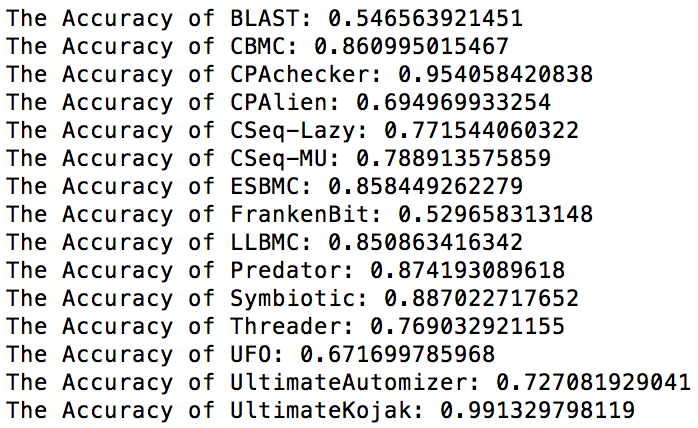
\includegraphics[width=3in]{figures/linear.PNG} &  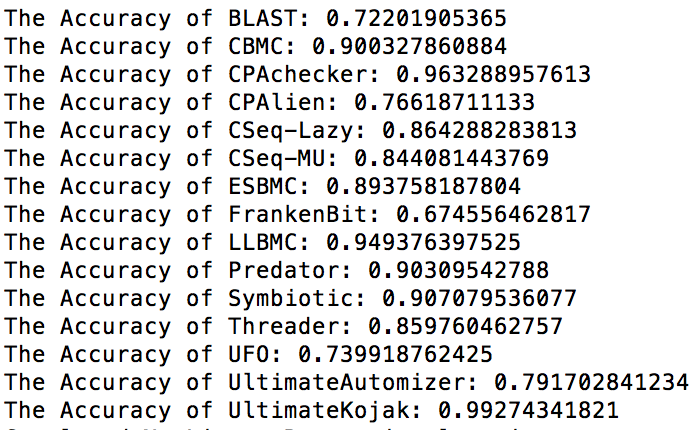
\includegraphics[width=3in]{figures/non_lin.PNG} \\ %
  \small (a) Basic linear regression  \label{fig:sub:lin} & 
  \small (b) Linear regression with non-linear transformation \label{fig:sub:non_lin}
\end{tabular}
\caption{Invariant violation in a virtual wallet example}
\label{fig:test_14}
\end{figure}
